%%%%%%%%%%%%%%%%%%%%%%%%%%%%%%%%%%%%%%%%%%%%%%%%%%%%%%%%%%%%%%%%%%%%%%%%%%%%%%%%
%               Capitulo 5: Descripción detallada del sistema                  %
%%%%%%%%%%%%%%%%%%%%%%%%%%%%%%%%%%%%%%%%%%%%%%%%%%%%%%%%%%%%%%%%%%%%%%%%%%%%%%%%

\chapter{Descripción detallada del sistema}
\label{chap:desc}

Una vez que se ha visto cuál es la arquitectura general del sistema y cómo se agrupan
y relacionan los diferentes módulos lógicos y componentes funcionales, vamos a pasar
a estudiar dichos elementos de manera más detallada, haciendo especial hincapié en los
componentes funcionales.

\section{Módulo de interacción con el usuario}

En este módulo, tal y como se comentó en el capítulo anterior, es donde se lleva a cabo
la interacción con el usuario. Aquí es donde el usuario define el dominio y crea el archivo
de configuración, que son los dos elementos que va a utilizar el sistema cuando entre en
funcionamiento. Más que un componente software dentro del sistema, este módulo representa un
proceso general que es llevado a cabo por el usuario, el cual le permite modificar directamente
el funcionamiento del sistema.

En la figura \ref{fig:iterative_waterfall_model} se puede ver qué pasos se llevan dentro de este
módulo lógico. Se comienza con la definición del dominio \texttt{PDDL} (\textit{Domain writing}), el cual
representará el juego. Después de ese proceso vendría la definición del archivo de configuración
(\textit{Configuration generation}). A la hora de crear dicho archivo, el usuario puede darse cuenta de que no ha
considerado ciertos elementos en su dominio, lo cual implicará que se deberán hacer ciertas modificaciones
sobre dicho dominio. Por último, con los dos ficheros ya creados, el usuario ejecutaría el sistema
(\textit{System execution}). En función de la salida obtenida, el usuario podría modificar o bien el
dominio creado para adaptarlo mejor al juego, o bien modificar el archivo de configuración para por ejemplo
establecer nuevos objetivos o corregir algún error a la hora de crearlo.

\begin{figure}[H]
    \centering
    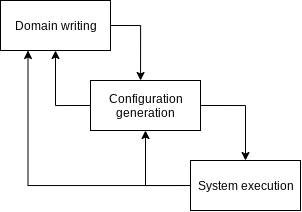
\includegraphics[scale=0.6]{img/CH05/iter_waterfall_model.png}
    \caption{Ciclo de vida dentro del módulo de interacción con el usuario.}
    \label{fig:iterative_waterfall_model}
\end{figure}

Visto este esquema, pasemos a estudiar las componentes funcionales que forman el módulo.

\subsection{Creación del dominio}

La creación del dominio de planificación es llevada a cabo completamente por el usuario.
Implica definir una representación del juego que incluya los elementos que se pueden
encontrar en éste, las acciones del agente (con sus precondiciones y efectos) y una serie de predicados
que definen el funcionamiento del juego. Dicho dominio, en la medida de lo posible, debería ser
lo más parecido posible al juego original, de manera que casi todo lo que se haga en el juego
se pueda hacer en el dominio.

\subsection{Creación de la configuración}

La creación del archivo de configuración, a diferencia de la creación del dominio, tiene cierto grado
de automatización. Se dispone de un \textit{script} que permite generar parte de ésta a partir del
dominio creado en el paso anterior del proceso (ver figura \ref{fig:iterative_waterfall_model}) y
de la definición en \texttt{VGDL} del juego. La otra parte la tendrá que generar el usuario.

La creación de la configuración será descrita con mucho maś detalle en el próximo capítulo,
donde se comentará el proceso y cómo es un archivo de configuración.

\section{Módulo de planificación}

El funcionamiento del módulo de planificación se explicó en el capítulo anterior. En resumen, el
módulo se encarga de gestionar los objetivos proporcionados por el usuario en el archivo de
configuración, de elegir un objetivo y de obtener un plan válido hasta dicho objetivo, asegurándose
además que el plan pueda ser interpretado por el entorno de juego. La figura \ref{fig:flux-planning}
ilustra el funcionamiento del módulo de forma resumida. En líneas generales, el funcionamiento del módulo está
totalmente automatizado, si bien es cierto que requiere que el usuario haya definido el dominio \texttt{PDDL}
y el archivo de configuración. Se comunica con el módulo de ejecución del plan y monitorización,
recibiendo de él una discrepancia en caso de que se haya producido y proporcionándole un plan válido
hasta el objetivo actual.

\begin{figure}[H]
    \centering
    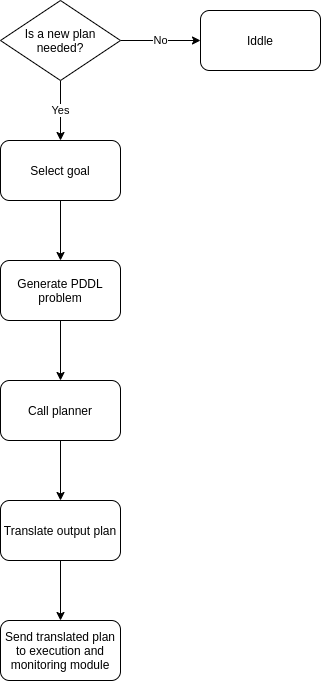
\includegraphics[scale=0.45]{img/CH05/flux_planning.png}
    \caption{Diagrama de flujo del módulo de planificación.}
    \label{fig:flux-planning}
\end{figure}

\subsection{Gestor de objetivos}
\label{sec:goal-manager}

La principal tarea de este módulo funcional es gestionar los objetivos que le han sido proporcionados
en el archivo de configuración y de establecer un objetivo actual. Para hacer dicha gestión, se almacenan
los objetivos en una estructura de datos similar a una agenda. Los objetivos están organizados
por prioridad, la cual indica si un objetivo debe completarse antes de que se intente buscar un plan
para otros objetivos, aunque esto se comentará con más detalle más adelante. Además de eso, un objetivo
puede estar en uno de los siguientes estados:

\begin{itemize}[label=\textbullet]
    \item \textbf{No planificado}: no se ha buscado ningún plan hasta ese objetivo.
    \item \textbf{Alcanzado}: el objetivo ha sido alcanzado satisfactoriamente.
    \item \textbf{Detenido}: el plan hasta el objetivo se ha detenido debido a una discrepancia.
    \item \textbf{Actual}: objetivo que ha decidido el gestor que debe alcanzarse.
\end{itemize}

La transición entre los distintos estados se puede ver en la figura \ref{fig:goal_transition}.
Un objetivo comienza en el estado no planificado (\textit{Not planned}), ya que no existe un plan
hasta dicho objetivo. Si es seleccionado, el objetivo pasa a ser el objetivo actual (\textit{Current goal}).
Estando en dicho estado, y tras haber obtenido un plan hasta él, si se alcanza dicho objetivo éste
pasa a estar alcanzado (\textit{Reached}). Si en cambio se produce una discrepancia, el objetivo pasa
a estar detenido (\textit{Preempted}). Desde dicho estado, el objetivo puede volver a ser
seleccionado como objetivo actual si se dan una serie de condiciones, como por ejemplo que
el objetivo detenido tiene que ser completado antes que cualquiera de los objetivos no planificados.
Es importante destacar que un objetivo puede pasar, debido a una discrepancia, desde el estado
no planificado o detenido al de alcanzado. Esto puede suceder si, mientras se está ejecutando el plan
hasta el objetivo actual, se alcanza accidentalmente algún objetivo que esté en este estado, debido
por ejemplo a los efectos de una acción.

\begin{figure}[H]
    \centering
    \scalebox{0.9}{
    \begin{tikzpicture}
        \node[Node style, state] (not_planned) {Not planned};
        \node[Node style, state, right of=not_planned] (current) {Current goal};
        \node[Node style, state, below of=not_planned] (reached) {Reached};
        \node[Node style, state,right of=reached] (preempted) {Preempted};
        
        \draw (not_planned) edge[above] node{Selected goal} (current)
              (not_planned) edge[left] node{Discrepancy} (reached)
              (current) edge[right, pos=0.2, bend left] node{Discrepancy} (preempted)
              (preempted) edge[left, pos=0.2, bend left] node{Selected goal} (current)
              (preempted) edge[above] node{Discrepancy} (reached)
              (current) edge node[left] {Plan completed} (reached);
    \end{tikzpicture}}
    \caption{Diagrama de transición del estado de un objetivo.}
    \label{fig:goal_transition}
\end{figure}

El módulo recibe como entradas los objetivos definidos por el usuario en el archivo de configuración,
y cuando sea el caso, una discrepancia que se ha producido a la hora de ejecutar el plan, proporcionada
por el monitor. La salida que genera es el objetivo actual, el cual es el nuevo objetivo para el que
el planificador debe obtener un plan. Esta salida se envía al generador de problemas, que se va a encargar
de generar un problema para ese objetivo.

\subsection{Generador de problemas}
\label{sec:problem-generator}

Este módulo funcional se encarga de generar los archivos de problema \texttt{PDDL} que necesita
el planificador. Recibe como entrada el objetivo actual que ha seleccionado el gestor de objetivos,
el estado del juego en formato \texttt{PDDL} del traductor de estados de observación y el nombre del
fichero de problema de salida y el nombre del dominio del archivo de configuración.

\subsection{Planificador}

El planificador tiene la tarea de obtener un plan desde el estado actual, representado en el problema
\texttt{PDDL}, hasta el objetivo actual. Podría decirse que este componente es el corazón tanto del módulo
lógico como de todo el sistema. Toda la arquitectura se ha montado alrededor de éste, con lo cual
eliminarlo haría que ésta fuese inútil.

Recibe como entradas el archivo con el dominio \texttt{PDDL} y el archivo de problema obtenido
por el generador de problemas. La salida que genera es un plan compuesto por acciones
\texttt{PDDL} hasta el objetivo, el cual se pasa al traductor de planes.

\subsection{Traductor de planes}
\label{sec:translate-plan}

Este componente funcional tiene la tarea de traducir los planes generados por el planificador,
los cuáles están formados de acciones \texttt{PDDL} a planes que sean interpretables por el entorno
de juego, es decir, planes formados por acciones \texttt{GVGAI}. Para cada una de estas acciones
se encarga de extraer también sus precondiciones y efectos instanciados, es decir, con los objetos
concretos del estado \texttt{PDDL} del juego. Esta información se puede utilizar luego en el monitor
para el estudio de las discrepancias.

El módulo funcional recibe como entrada el plan obtenido por el planificador y la correspondencia
entre acciones \texttt{PDDL} y \texttt{GVGAI}, la cual proviene del fichero de configuración. Genera
como salida el plan traducido a acciones de \texttt{GVGAI} junto con las precondiciones y efectos
instanciados de cada acción del plan. Dicha salida es enviada al ejecutor del plan.

\section{Módulo de ejecución del plan y monitorización}

El funcionamiento general del módulo fue puesto de manifiesto en el capítulo anterior. En resumidas
cuentas, este módulo lógico se encarga de ejecutar el plan obtenido por el módulo de planificación
y de monitorizar dicha ejecución, de manera que se detecten las discrepancias que se puedan producir.
El funcionamiento de este módulo está totalmente automatizado, aunque tal y como pasaba en el módulo
anterior, se requiere del archivo de configuración creado por el usuario. Se utiliza la información
de dicho fichero para automatizar la traducción de los estados de observación del juego a estados
\texttt{PDDL}. Se comunica con el módulo de planificación para comunicarle una discrepancia
y para recibir de él el plan a ejecutar.

\subsection{Motor del juego}

Este es el componente que visualiza y ejecuta el juego. En cada turno del juego, se obtiene a partir de él un
estado de observación, el cual representa el estado actual del juego. Dicha salida es utilizada por el
traductor del estado de observación. Además de eso, en cada turno recibe una acción del ejecutor del plan,
que es la que va a ejecutar el agente.

\subsection{Traductor del estado de observación}
\label{sec:translate-state}

La finalidad de este módulo funcional es generar, a partir de un estado de observación obtenido del
motor del juego, una representación en formato \texttt{PDDL} del estado de juego actual. Para poder
hacer esto de forma automática necesita, aparte de recibir como entrada el estado de observación del
motor del juego, una correspondencia entre los elementos y los predicados \texttt{PDDL} correspondientes,
la cual proviene del archivo de configuración que ha definido el usuario. La salida que produce,
el estado de juego en formato \texttt{PDDL}, es enviada al monitor y, en caso de que éste detecte
una discrepancia, al generador de problemas.

\subsection{Monitor}

El monitor se encarga de supervisar la ejecución del plan, detectando en el proceso si se ha producido
alguna discrepancia. Como se ha comentado anteriormente, una discrepancia se produce cuando el estado
actual del juego no es el esperado debido a que ha sucedido algún evento impredecible dentro del juego.
Con ``estado esperado'' nos referimos al que se indica en las precondiciones de la acción, ya que
éstas se tienen que satisfacer para que dicha acción pueda ser ejecutada.

De esta forma, el monitor recibe como entrada el estado del juego en formato \texttt{PDDL} del
traductor de estados de observación y las precondiciones y los efectos de la acción a ejecutar
del ejecutor del plan. Si no hay ninguna disconformidad entre las precondiciones y el estado del juego,
el monitor le indica al ejecutor que puede proceder. Si en cambio hay algún tipo de disconformidad,
el monitor detendría la ejecución del plan e indicaría al gestor de objetivos que se ha producido
una discrepancia, de forma que se tendría que seleccionar un nuevo objetivo y buscar un plan hasta
él. Adicionalmente, con los efectos de la acción se puede determinar si un objetivo se ha alcanzado
antes de tiempo (también de forma accidental). Esto también generaría una discrepancia, ya que no se
esperaba que se alcanzase un objetivo antes de tiempo. Sin embargo, esta discrepancia no obligaría
a detener la ejecución del plan actual. Lo único que haría sería indicarle al gestor de objetivos
que marque como alcanzado el objetivo alcanzado antes de tiempo. Todo el procedimiento que acaba de describirse
puede verse en la figura \ref{fig:flux-monitor}.

\begin{figure}[H]
    \centering
    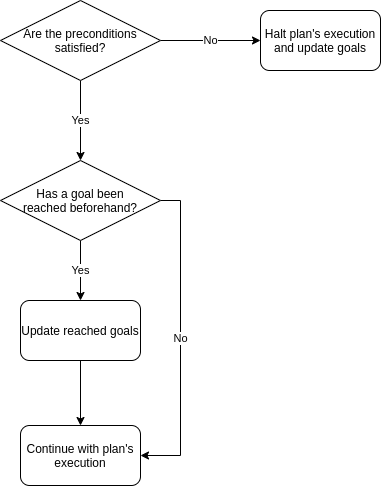
\includegraphics[scale=0.45]{img/CH05/flux_monitor.png}
    \caption{Diagrama de flujo del funcionamiento del monitor.}
    \label{fig:flux-monitor}
\end{figure}

\subsection{Ejecutor del plan}

Este módulo se encarga de ejecutar el plan que le ha sido proporcionado por el módulo de planificación.
En cada turno se tiene que ejecutar una acción de dicho plan. No obstante, antes de eso hace falta
comprobar que el estado de juego actual es el correcto y no se ha producido ninguna discrepancia, ya
que en caso contrario el plan dejaría de ser válido. De esta parte se encarga el monitor, el cual
le comunica si todo está en orden o no.

Por tanto, este componente recibe como entrada el plan del traductor de planes y envía al monitor
las precondiciones y los efectos de la acción que va a ejecutar a continuación. Si no hay ningún
tipo de problema, el ejecutor del plan manda al motor de juego la siguiente acción que se
tiene que ejecutar.
